\documentclass[12pt,a4paper]{article}

\usepackage[english]{babel}
\usepackage[margin=2.5cm]{geometry}
\usepackage{graphicx}
\usepackage[T1]{fontenc}
\usepackage{hyperref}
\usepackage{pdfpages}

\begin{document}

\begin{titlepage}
    \begin{center}
        \vspace*{\fill}
        {\Large\bfseries FIT VUT v Brně}\\[3mm]
        {\large 2026/2027}\\[12mm]

        {\Huge\bfseries Project IFJ/IAL}\\[12mm]

        {\large\bfseries Authors \& Point Distribution:}\\[4mm]

        \bgroup
        \def\arraystretch{1.3}
        \begin{tabular}{l l l l}
            \textbf{Mykhailo Barkovskyi} & xbarkom00 & 282787 & 25\% \\
            Lukáš Zeleňák & xzelenl00 & 282620 & 25\% \\
            Lukáš Bela & xbelalu00 & 281720 & 25\% \\
            Juraj Pauček & xpaucej00 & 281716 & 25\% \\
        \end{tabular}
        \egroup
        \\[12mm]

        {\large\bfseries Chosen variant:} TRP-izp\\[6mm]

        {\large\bfseries Implemented extensions:} None\\[6mm]

        {\large\bfseries Git repository link:}\\[2mm]
        \url{https://github.com/michael-b-gh/IFJ26-xbarkom00}\\[2mm]
        \vfill

        {\large Submission date: \today}
    \end{center}
\end{titlepage}

\newpage
\tableofcontents
\newpage
\section{Work distribution}
\begin{itemize}
  \item Team lead, parser, precedence analysis, Makefile, error, scanner header files and documentation completion: Mykhailo Barkovskyi
  \item Generator: Lukáš Bela
  \item Lexical analysis, error and scanner header files: Juraj Pauček
  \item Symtable, hashtable, semantic, tokenBuffer, Makefile, tests: Lukáš Zeleňák
\end{itemize}

\section{Development and collaboration}
\subsection{Collaboration and code review}
Team was created at 1st week of semester, Discord was used as main platform for communication. Every week, we had short (about 10 minutes) Friday calls at 15:30, where we were establishing what to do and exchanging opinions, with presence almost 90\%. We were working continuosly, frontend of parser was ready week before main submission deadline. Github was chosen as version system, every member was working in his own branch. Before integration, team lead controled written code to specification and returned list of fixes.
\subsection{Testing}
More than three hundred black-box tests with ic26int were used to test basic functionality of program. 
\subsection{Code formatting}
Clang-format with basic LLVM style ensured standard of formatting through all source files. 

\section{Compiler architecture}
Source code (IFJ26) goes from standard input to Lexer, that stores lexems to tokens, provides lexical analysis and stores tokens in TokenBuffer. Parser and Expression use it for syntax analysis through 3 passes (1st pass is syntax control and function heads registration, 2nd pass is semantic controls and 3rd is code generation). Parser checks type with help of Semantic (using DType, \texttt{check\_*} functions). Semantic sends Symbol * to symbol table, SymTable represents every opened scope (block) as 1 instance of Hashtable (key is name of identifier char * and value Symbol * stored as void *). Finally, Parser and Expression begin code generating using codegen functions to emit target code (IFJcode26) to standard output.


\begin{center}
   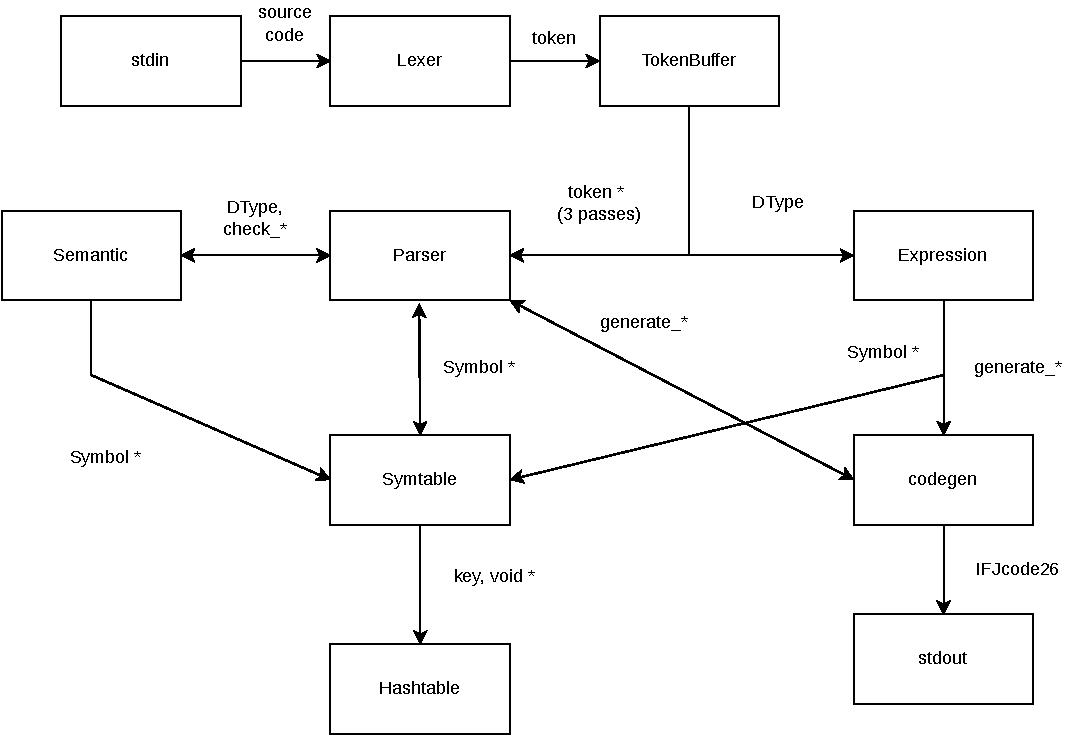
\includegraphics[width=0.95\textwidth]{architecture.pdf}
\end{center}


\section{Lexical analysis}     
The lexical analyzer is implemented as finite-state machine (FSM). It is driven by state variable \texttt{state} inside \texttt{get\_next\_token} function. Lexical analyzer uses function \texttt{NextSymbol} to get symbols from standard input sequentially. It stores lexemes in dynamically allocated array \texttt{word}. After recognizing valid lexeme, it assigns type of lexeme into \texttt{token\_type} and content into \texttt{attribute} within 
\texttt{token} structure.
\subsection{Deviations}
Because IFJ26 language for example uses indentation-based blocks lexical analyzer deviates from theoretical FSM in ways such as:
\begin{itemize}
    \item \textbf{Indentation tracking}\\
    Because IFJ26 uses indentation-based blocks of code, before entering main FSM on each new line \texttt{new\_line=1} of code, lexical analyzer counts leading spaces and compares them with top of indentation stack \texttt{dent\_arr}, so it can generate \texttt{TOKEN\_IND}, \texttt{TOKEN\_DED} or no token if indentation level hasn't changed. In case of parentheses \texttt{parent\_count>0} it only checks if the indentation level inside is greater than indentation level of preceding block.  
    \item \textbf{Character pushback}\\
    In some states one extra character is needed so the FSM can decide whether to continue in current lexeme or to generate token. In states that do not need this extra character or in token generating states, this extra character is returned via \texttt{ungetc} function.
    \item \textbf{Escape sequence translation}\\
    Escape sequences such as \texttt{\textbackslash{}n} or \texttt{\textbackslash{}t} in single-line strings \texttt{STATE\_STRING} are translated into their corresponding control characters during reading of the lexemes.
    \item \textbf{Keywords and directive control}\\
    Neither keywords nor directive \texttt{@main} have their own states but are compared in \texttt{STATE\_ID} and \texttt{STATE\_START} respectively using \texttt{strcmp} function.
    \item \textbf{Memory extensions of FSM}\\
    Since normal FSM cannot support infinite indentation levels or infinite levels of comment nesting, lexical analyzer uses external memory structures: \texttt{counter} and \texttt{dent\_arr} for indentation and \texttt{comm\_counter} for nested comments.
\end{itemize}

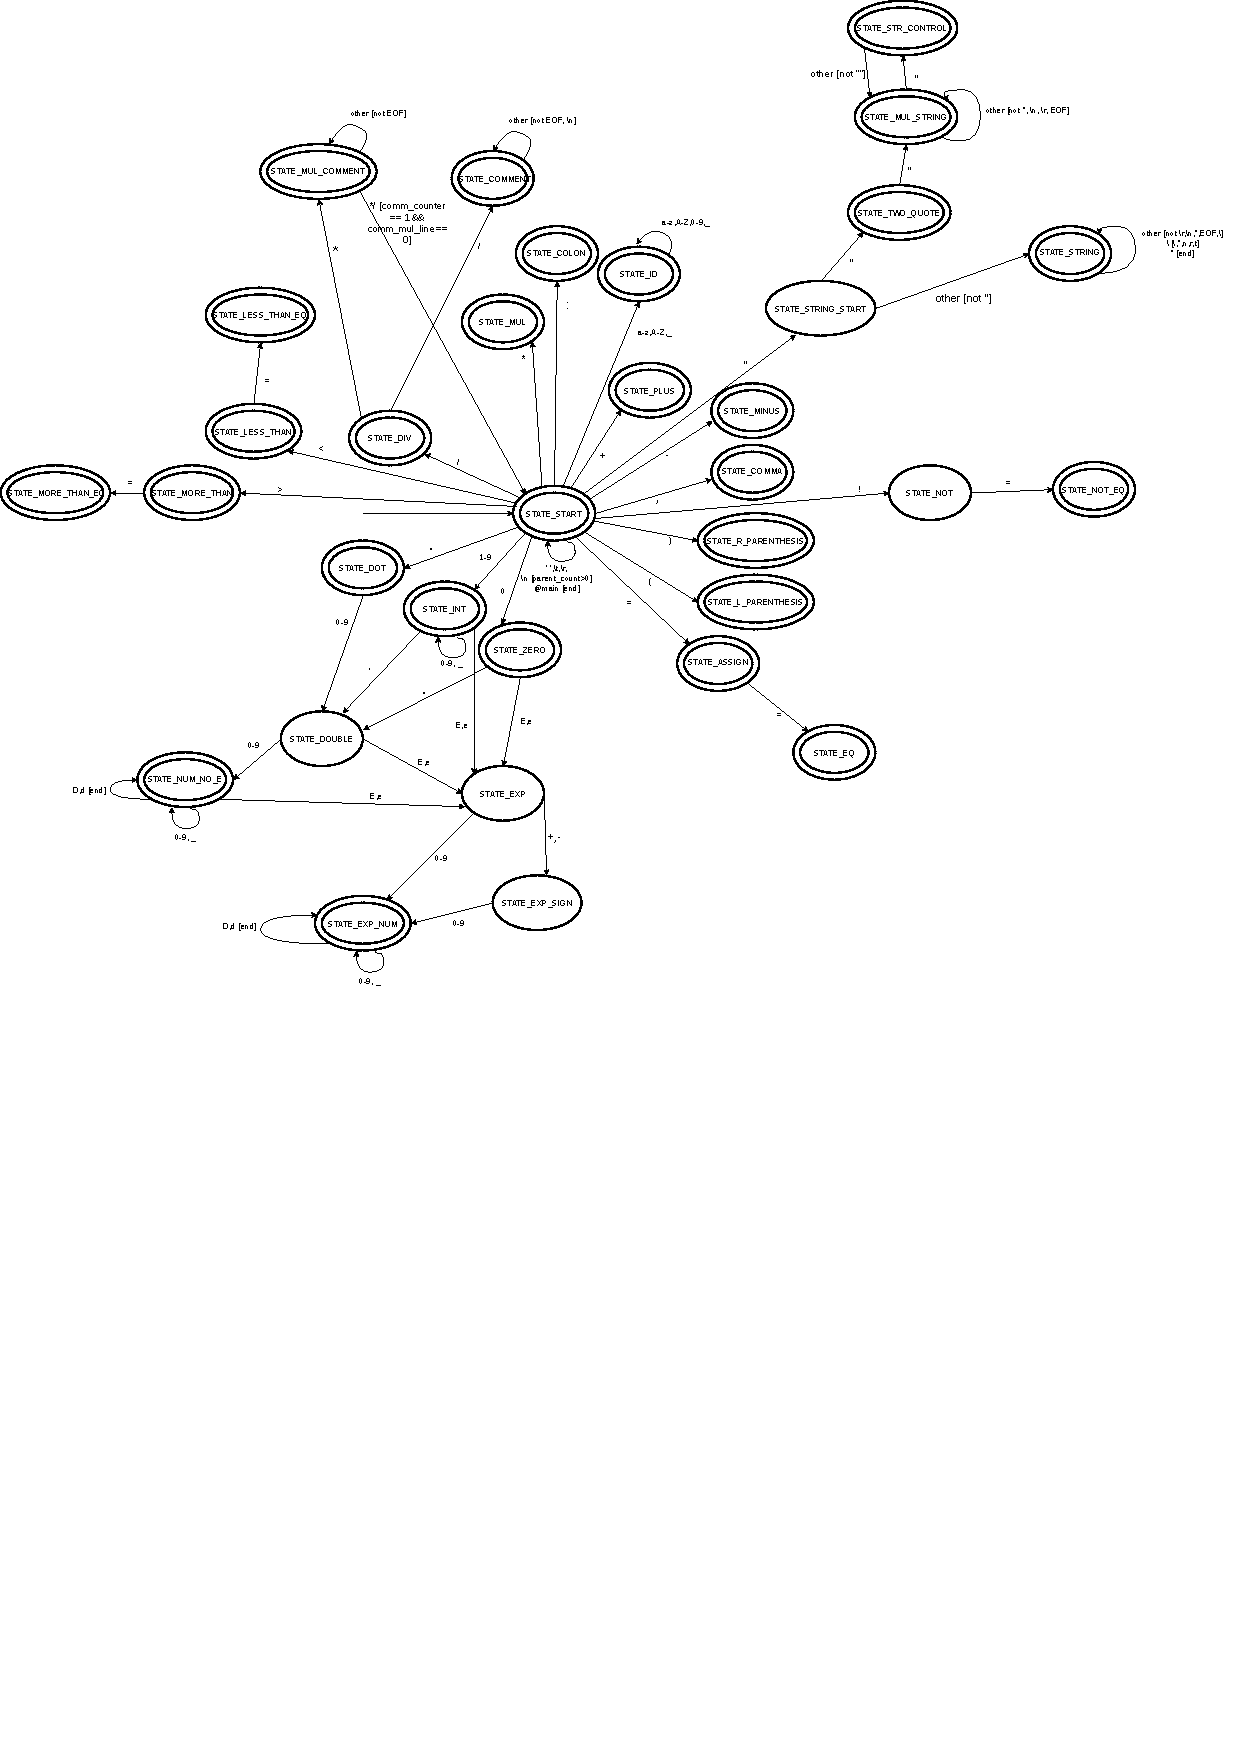
\includepdf[pages=1]{FSM_COMPLETE_5-1.pdf}

\section{Token Buffer}          
Before parsing, all tokens are loaded up to EOF into a dynamic array (initial capacity 100, doubling when full). This gives the parser random access by index to jump to positions like \texttt{bodyStartIdx} when inferring return types or handling forward function calls.

\section{Syntactic analysis}      
\subsection{LL grammar}
\begin{verbatim}
1) <start> -> <prolog> <top_list> EOF
<top_list> -> <function> <top_list> | <main> <top_list> | EOL <top_list> | eps
2) <prolog> -> import id . * EOL
3) <main> -> @main <function>
4) <var_def> -> val/var id [: <type>] = <expr_or_call> EOL
5) <function> -> def id (<param_list>) [: <type>] = <expr_or_call> EOL | EOL <block>
6) <if> -> if <expr> then EOL <block> else EOL <block>
7) <while> -> while <expr> do EOL <block>
8) <type> -> Int | Double | String | Unit 
9) <param_list> -> eps | id: <type> (, : <type>)*
10) <block> -> IND <stmt_list> DED 
<stmt> -> <var_def> | <if> | <while> | <return> 
| id = <expr_or_call> EOL | <expr_or_call> EOL | EOL
11) <return> -> return [<expr_or_call>] EOL
12) <expr_or_call> -> <func_call> | <expr> 
13) <func_call> -> id (<arg_list>) 
<arg> -> () | id | int | double | string

\end{verbatim}

\subsection{LL table}
We use lookahead \texttt{peek\_type(buf, idx)} to distinguish between assign (id = ...), function call (id(...)), expression, and () (Unit) in arguments. 

\begin{table}[h!]
\centering
\scriptsize
\begin{tabular}{|l|c|c|c|c|c|c|c|c|c|c|c|c|}
\hline
Non-terminal / Token & \texttt{import} & \texttt{def} & \texttt{@main} & \texttt{val/var} & \texttt{if} & \texttt{while} & \texttt{return} & \texttt{id} & \texttt{type} & \texttt{IND} & \texttt{DED} & \texttt{EOL/EOF} \\ \hline
$\langle start \rangle$          & 1 &   &   &   &   &   &    &    &   &    &   &   \\ \hline
$\langle prolog \rangle$         & 2 &   &   &   &   &   &    &    &   &    &   &   \\ \hline
$\langle main \rangle$           &   &   & 3 &   &   &   &    &    &   &    &   &   \\ \hline
$\langle var\_def \rangle$       &   &   &   & 4 &   &   &    &    &   &    &   &   \\ \hline
$\langle function \rangle$       &   & 5 &   &   &   &   &    &    &   &    &   &   \\ \hline
$\langle if \rangle$             &   &   &   &   & 6 &   &    &    &   &    &   &   \\ \hline
$\langle while \rangle$          &   &   &   &   &   & 7 &    &    &   &    &   &   \\ \hline
$\langle type \rangle$           &   &   &   &   &   &   &    &    & 8 &    &   &   \\ \hline
$\langle param\_list \rangle$    &   &   &   &   &   &   &    & 9  &   &    &   &   \\ \hline
$\langle block \rangle$          &   &   &   &   &   &   &    &    &   & 10 &   &   \\ \hline
$\langle return \rangle$         &   &   &   &   &   &   & 11 &    &   &    &   &   \\ \hline
$\langle expr\_or\_call \rangle$ &   &   &   &   &   &   &    & 12 &   &    &   &   \\ \hline
$\langle func\_call \rangle$     &   &   &   &   &   &   &    & 13 &   &    &   &   \\ \hline

% Sem doplň řádky pro své neterminály a čísla pravidel
\end{tabular}
\end{table}
\subsection{Precedence table}
\begin{table}[h!]
\centering
\begin{tabular}{|l|c|c|c|c|c|c|c|c|c|}
\hline
 & \texttt{*,/} & \texttt{+,-} & \texttt{rel} & \texttt{==,!=} & \texttt{(} & \texttt{)} & \texttt{i} & \texttt{un.+,-} & \texttt{\$} \\ \hline
\texttt{*,/}    & $>$ & $>$ & $>$ & $>$ & $<$ & $>$ & $<$ & $<$ & $>$ \\ \hline
\texttt{+,-}    & $<$ & $>$ & $>$ & $>$ & $<$ & $>$ & $<$ & $<$ & $>$ \\ \hline
\texttt{rel}    & $<$ & $<$ &     & $>$ & $<$ & $>$ & $<$ & $<$ & $>$ \\ \hline
\texttt{==,!=}  & $<$ & $<$ & $<$ &     & $<$ & $>$ & $<$ & $<$ & $>$ \\ \hline
\texttt{(}      & $<$ & $<$ & $<$ & $<$ & $<$ & $=$ & $<$ & $<$ &     \\ \hline
\texttt{)}      & $>$ & $>$ & $>$ & $>$ &     & $>$ &     &     & $>$ \\ \hline
\texttt{i}      & $>$ & $>$ & $>$ & $>$ &     & $>$ &     &     & $>$ \\ \hline
\texttt{un.+,-} & $>$ & $>$ & $>$ & $>$ & $<$ & $>$ & $<$ & $<$ & $>$ \\ \hline
\texttt{\$}     & $<$ & $<$ & $<$ & $<$ & $<$ &     & $<$ & $<$ &     \\ \hline
\end{tabular}
\end{table}

Precedence table is based on table from IFJ chapter 8. Unary operator is detected by checking of stack top: if there is non-terminal E, operand i or right parenthesis, it is binary operator. Else it is unary operator with the biggest priority and right associativity. Reduction works in this way: parser counts number of symbols after \texttt{ITEM\_MARKER} and reduces them to non-terminal E. If there is 1 element, it is identifier of variable or literal, if 2 it is literal Unit type or unary operator; if there is 3 elements, it is parenthesized expression, binary arithmetic or relation operators.

\section{Symbol Table}           

\subsection{Hash Table}
We chose the TRP-izp variant using implicit chaining (open addressing). All items are stored directly in a single array without using linked lists. When a collision occurs, the algorithm simply finds another unused slot within the same array.

Each hash table item consists of a key (an owned copy of the identifier name), a value \texttt{void *}, and a boolean flag indicating whether the slot is used. We chose the djb2 hash function \cite{djb2} because of its minimal code, high speed, and good string distribution.

The starting index is calculated as hash \% \texttt{table->size}. If the slot is occupied by a different key, the algorithm shifts right by one position, wrapping around to the start of the array when reaching the end. If the same key is already present in the array, it returns \texttt{HASHTABLE\_ITEM\_EXISTS}. Once an unused slot is found, the item is stored there.

The initial capacity of the table is 100. Before inserting a new item, we check if the load factor would exceed 0.7. If it does, the table resizes to double its current capacity. After resizing, all existing items are rehashed because their indexes depend on the table size. 

\subsection{Symbol Table Interface}
The symbol table is implemented as an abstract data type built on top of the hash table. The rest of the compiler interacts with it exclusively through the symbol table interface. Each hash table item stores a pointer to a \texttt{Symbol} structure inside its \texttt{void *} value field, which keeps the hash table completely generic and unaware of the \texttt{Symbol} type.

The symbol table is a stack of scopes implemented as a dynamic array of hash tables. \texttt{scopes[0]} is the global scope holding user functions and 10 built-in functions inserted upon initialization. Entering a block pushes a new scope, and exiting frees it along with its symbols.

Lookup searches from the innermost scope outward, enabling variable shadowing. Insertion targets only the current scope. When the hash table returns \\ \texttt{HASHTABLE\_ITEM\_EXISTS}, the symbol table returns \texttt{NULL}, which \texttt{check\_variable\_def} translates into \texttt{REDEF\_SEM\_ERR} for the parser to report as error 4, while reusing the name in an inner block remains allowed.

\texttt{Symbol} is structure that is saved in symbol table:
\begin{itemize}
  \item If it is variable then \texttt{isMutable} (\texttt{val}/\texttt{var})
  \item If it is function then \texttt{paramTypes} and \texttt{returnType}, \texttt{bodyStartIdx} (index to the token buffer where the body starts), \texttt{inferState} (for inference of return type and detection of untyped recursion both in functions without an explicit return type)
\end{itemize}

When the parser jumps into another function's body to infer its return type, all local scopes are temporarily saved, leaving only the global scope active, and restored upon return.

\section{Semantic Analysis}      
Semantic checks are called directly by the parser during syntax analysis, returning a type or status code while the parser reports errors. \texttt{DTYPE\_UNKNOWN} marks an invalid result, and the only implicit conversion (\texttt{DTYPE\_INT} $\rightarrow$ \texttt{DTYPE\_DOUBLE}) is handled centrally in \texttt{is\_type\_compatible}. Variable definitions, assignments, and function calls are validated against the symbol table for mutability, types, and argument counts. Functions without an explicit return type have their type inferred, while untyped recursion is detected via \texttt{inferState} (error 6).

\section{Code Generation}         
\subsection{The code generator}
The code generator is a module to generate intermediate code / target language \texttt{IFJcode26}. The
module consists of codegen.h and codegen.c and is implemented as a set of functions emitting the
generated code to standard output using printf commands.

\subsection{The start of a module}
The module begins with the mandatory opening line .IFJcode26. Then it generates
CREATEFRAME for the skeleton main followed by declaring global variables GF@tmp1 and GF@tmp2
for further use. After this, the @main function calls itself and ends with EXIT int@0 since the @main
can have any name and the interpret cannot fall into bodies of other functions.

\subsection{Stack instructions}
Stack instructions work with a stack and usually with pushed variables. The result is on top of a stack.
The module includes most of the stack instructions from instruction set in the specification of
languages IFJ26 a IFJcode26 and are generated by calling a function which is named after said stack
instruction. Most of these instructions have only one line of printf command and without parameters
(POPS, ADDS, MUL) because the variables are expected to be in the stack.

The \texttt{GENERATE\_CONCATS} function in the module is not a part of a stack instruction in the
specification. Instead it works with global variables. Variables from a stack are popped into global
variables, executes non-stack instruction CONCAT and the result is pushed 

\subsection{Generation functions}
At the start of each function, a new local frame is created and pushed onto the frame stack using
CREATEFRAME and PUSHFRAME. If the function needs parameters, they are popped for the stack into
local variables, which are created using \texttt{DEFVAR LF@<name>}.

The function ends with instructions POPFRAME followed by RETURN. If the function returns a variable
before it generates said instructions, the variable is pushed into the stack using \texttt{PUSHS LF@<name>}
or the result is already in the stack.

\subsection{Built-in functions}
Built-in functions are functions that are generated completely without need to call other functions.
They are created at the end of the module and each has a specific task, parameters and return values
said in the specification. Some of them are variations of an instruction in the instruction set, some of
them are more complicated. All built-in functions work with the stack and have their own label.

\subsection{if/else and while}
The if/else condition and while cycle have each their 3 own functions to generate. For if/else
condition functions are for the start, the ELSE part (if it has) and the end. For while cycle functions are
for the start, the condition and the end. Each if/else and while needs its own label so the module has
static id counter for each of them.

\section{Module description}
\begin{itemize}
\item Lexer.c / scanner.h -- finite automaton with stack IND/DED level and definition of token structure
\item token\_buffer.c / token\_buffer.h -- dynamically allocated array of all tokens size from stdin (so parser can do several passes)
\item parser.c -- Recursive Descent of 3 passes and enter point main
\item expression.c / expression.h -- Precedence analyze on stack with 2D precedence table, type controls and generation of stack functions
\item semantic.c / semantic.h -- control of type compatibility of terms, assigns, parameters in call, returning values and \texttt{@main} signature
\item symtable.c / symtable.h -- symbol table made as stack of hash tables for inner scope, storing built-in functions and giving unique IDs to local variables
\item hashtable.c / hashtable.h -- \texttt{TRP-izp} with linear probing, hash-function DJB2 and automatic double increasing of capacity if full on 70\%
\item codegen.c / codegen.h -- emits (prints) target code \texttt{IFJcode26} to stdout (uses stack, frames LF/GF, unique labels for \texttt{if/while} and bodies of built-in functions)
\item error.h -- definition of compiler returning code macros
\end{itemize}

\section{AI}
\subsection{Lukáš Zeleňák}

I wrote the compiler code assigned to me (hash table, symbol table, semantic analysis, and token buffer) myself. I used AI (Claude Opus) for code reviews, to explain concepts I did not understand or to improve comments in header files. I also used AI to generate unit tests for the finished hash table and symbol table, which helped uncover memory leaks, as well as black-box tests for whole compiler. However, there were some issues with the AI output. For example, it used non-existent token in the tests, which prevented compilation until I fixed them. In another case, it generated a test expecting \texttt{NULL} on a \texttt{malloc} failure, which failed with exit code 99 because our team convention is to call \texttt{exit(INT\_ERR)}. I rejected this test and removed it.

\subsection{Juraj Pauček}

I used AI (ChatGPT/Gemini) as consultant in way where I had some my idea and checked if it is optimal to do in this way or what tools C language provide to use for kind of things etc. All AI generated fragments related to me in source code are commented.

\subsection{Mykhailo Barkovskyi}

I used AI (Google Gemini Pro/Argon) for architectonic consultations (Socratic approach), to explain some parts of specification to prevent misunderstandings, sometimes for debugging, for code review, to structurize our calls. Model I used has restricted code generation, Recursive Descent and Operator-Precedence Parser architecture is based on slides 7 and 8 IFJ. I used it with cold head, for example, when I worked on block end control, AI suggested C-style logic (where dead code type after \texttt{return} doesn't matter), I compared it with specification, rejected it, and wrote \texttt{parse\_block} and \texttt{parse\_if} in right way.

\subsection{Lukáš Bela}

I used AI (Gemini Auto) for explaining specification itself, when I didn't understand some part and for commit-writing inspiration.

\section{References}
\begin{thebibliography}{9}
\bibitem{djb2}
  O.~Yigit. \emph{Hash Functions} [online]. York University.
  Available at: \url{http://www.cse.yorku.ca/~oz/hash.html} [2026-11-20].
\bibitem{ifj26spec}
  O.~Ondryáš, Z.~Křivka. \emph{Specifikace jazyků IFJ26 a IFJcode26 (IFJ/IAL 2026/2027)}. FIT VUT v Brně, rev. 2026-10-11.
\bibitem{ifjlectures}
  A.~Meduna, R.~Lukáš. \emph{Formální jazyky a překladače (IFJ) -- lecture slides}. FIT VUT v Brně, 2026.
\bibitem{iallectures}
  I.~Burgetová, R.~Hranický. \emph{Algoritmy (IAL) -- lecture slides}. FIT VUT v Brně, 2026/2027.
\end{thebibliography}

\end{document}